% !TeX spellcheck = cs_CZ
\wikitextrule
\begin{example}\label{mai:exam070}
  \textbf{Kolik rychlostí má molekula plynu}\newline\small
  Tato otázka se zdá na první pohled zcela nesmyslná. Každý student fyziky ví, že molekuly plynu 
  lze popisovat jako klasické částice, jejichž mechanický stav je jednoznačně určen polohovým 
  vektorem a vektorem rychlosti. Molekula má tedy vždy určitou hodnotu rychlosti. Představte si ale 
  takový plyn ve skutečnosti. Jeden mol jeho látkového množství (např. pro kyslík to představuje 
  hmotnost \num{32} gramů) obsahuje asi \num{6.623e23} molekul! Kdybychom chtěli plyn popisovat 
  jako soustavu klasických částic v mechanice, museli bychom v daném okamžiku znát polohu a 
  rychlost každé molekuly z tohoto obrovského počtu. A to je principiálně nemožné, protože do 
  chování takové soustavy zasahuje velmi podstatným způsobem „náhoda“. Nemůžeme určit, ve kterém
  bodě prostoru právě daná molekula je a jak rychle se pohybuje. Dokážeme pouze určit, s jakou 
  pravděpodobností se nachází v elementárním objemu \(\Delta V = \Delta x \Delta y \Delta z\) v 
  okolí daného bodu o polohovém vektoru \(\vec{r}\) a s jakou pravděpodobností \(\Delta P\) leží 
  koncový bod vektoru její rychlosti v elementárním objemu \(\Delta\Omega = \Delta v_x \Delta v_y 
  \Delta v_z\) „rychlostního“ prostoru v okolí zadané rychlosti \(\vec{v}\). Uvažujme o 
  nejjednodušším modelu plynového tělesa, takzvaném ideálním plynu, jehož molekuly jsou stejné a 
  navzájem neinteragují s výjimkou kratičkých náhodných srážek. Molekuly takového plynu jsou z 
  hlediska pravděpodobnostního popisu navzájem ekvivalentní. Pravděpodobnost \(\Delta P\) bude pro 
  všechny stejná a pro velmi malé elementární objemy bude dána vztahem
  \begin{equation*}
    \Delta P(\vec{r},\vec{v}) = \varrho(\vec{r},\vec{v})\Delta V \Delta\Omega,
  \end{equation*}
  kde \(\varrho(\vec{r},\vec{v}) = \varrho(x, y, z, v_x, v_y, v_z)\) je odpovídající hustota 
  pravděpodobnosti. Jak ale hustota konkrétně závisí na polohách a rychlostech molekul? Tento 
  fyzikální zákon, zvaný \textbf{Gibbsovo rozdělení}, se řídí exponenciální funkcí
  \begin{equation*}
    \varrho(\vec{r},\vec{v}) = K\exp\left(-\dfrac{E(\vec{r},\vec{v})}{kT}\right)
  \end{equation*}
  kde \(E\) je \textbf{mechanická energie molekuly} (kinetická plus potenciální v případném silovém 
  poli), \(T\) je \textbf{absolutní teplota plynu} udávaná v kelvinech a \(k = 
  \SI{1.38e-23}{\joule\per\kelvin}\) je \textbf{Boltzmannova konstanta}.
  
  Zajímá-li vás, proč si příroda v tomto případě vybrala zrovna exponenciální funkci, sledujte 
  následující orientační úvahu: Rozdělme si v myšlenkách plynové těleso na dvě části, jimž 
  odpovídají energie \(E_1\) a \(E_2\). Celková energie soustavy je \(E = E_1 + E_2\). Označme 
  \(P(E)\) pravděpodobnost, že, se soustava nachází ve stavu s energií \(E\), pravděpodobnosti, že 
  se jednotlivé části nachází nezávisle ve stavech s energiemi \(E_1\) a \(E_2\), pak jako
  \(P(E_1)\) a \(P(E_2)\). Pravděpodobnost, že se první část soustavy nachází ve stavu s energií 
  \(E_1\) a \textbf{současně} druhá část ve stavu s energií \(E_2\), je rovna součinu 
  pravděpodobností těchto nezávislých jevů. Proto \(P(E_1 + E_2) = P(E_1) \cdot P(E_2)\). Tuto 
  vlastnost mají ovšem právě exponenciální funkce. Platí tedy \(\varrho \approx\exp(\beta E)\). 
  Konstantu \(\beta\) určí jen experiment, z něhož vychází \(\beta = - (kT)^{-1}\).
  
  Vrátíme se nyní k výchozímu problému, neboť úvodní otázka nabyla smyslu: Molekula může mít 
  libovolnou rychlost s větší či menší pravděpodobností. Nebude-li ideální plyn umístěn v žádném 
  silovém poli, bude mechanická energie molekuly dána pouze energií kinetickou. Elementární 
  pravděpodobnost, že koncový bod rychlosti molekuly leží v elementárním objemu \(\Delta\Omega\) v 
  okolí bodu \(\vec{v}\) „rychlostního“ prostoru, bez ohledu na to, v jaké části „obyčejného“, tj. 
  \textbf{konfiguračního prostoru} se vyskytuje, je
  \begin{equation*}
    \Delta P(\vec{v}) = \varrho(\vec{v})\Delta\Omega 
                      = C\exp\left(-\dfrac{m(v_x^2 + v_y^2 + v_z^2)}{2kT}\right)\Delta\Omega.
  \end{equation*}
  Tato pravděpodobnost, jak je vidět, nezávisí na směru rychlosti, pouze na její velikosti, 
  \(\varrho(\vec{v}) = \varrho(v)\). Konstantu \(C\) určíme snadno. Pravděpodobnost, že molekula má 
  vůbec nějakou rychlost, je rovna jedné (jistý jev). Matematický zápis této skutečnosti vyžaduje 
  znalost takzvaného trojného integrálu (integrujeme podle tří proměnných  - složek vektoru 
  rychlosti). V našem případě se však výpočet redukuje na součin tří integrálů jednoduchých,
  \begin{equation*}
    \int_{\Omega}\varrho(v_x, v_y, v_z)\dd{v_x}\dd{v_y}\dd{v_z} = 1
  \end{equation*}
  \begin{equation*}
    \Rightarrow C \cdot
     \int_{-\infty}^{\infty}\exp\left(\dfrac{mv_x^2}{2kT}\right)\dd{v_x} \cdot
     \int_{-\infty}^{\infty}\exp\left(\dfrac{mv_y^2}{2kT}\right)\dd{v_y} \cdot
     \int_{-\infty}^{\infty}\exp\left(\dfrac{mv_z^2}{2kT}\right)\dd{v_z} =1.
  \end{equation*}
  Po substitucích \(mv_i^2/2kT = u^2,\, i = x, y, z\) vede výpočet na \textbf{Laplaceův integrál}
  \begin{equation*}
    \int_{-\infty}^{\infty}\exp(-u^2)\dd{u} = \sqrt{\pi}.
  \end{equation*}
  Dostáváme
  \begin{equation*}
    C = \left(\dfrac{m}{2\pi kT}\right)^{\frac{3}{2}} \Rightarrow
    \Delta P(\vec{v}) = \left(\dfrac{m}{2\pi kT}\right)^{\frac{3}{2}}
                        \exp\left(- \dfrac{mv^2}{2 kT}\right)\dd{v_x}\dd{v_y}\dd{v_z}
  \end{equation*}
  Hustota pravděpodobnosti je stejná pro všechny koncové body vektoru rychlosti \(\vec{v}\) ležící 
  v rychlostním prostoru na kulové ploše o poloměru rovném velikosti rychlosti \(v\). Jaká bude 
  elementární pravděpodobnost \(\Delta P(v)\), že molekula má velikost rychlosti v intervalu \((v, 
  v + \Delta v)\) bez ohledu na směr pohybu? Tuto pravděpodobnost dostaneme, vezmeme-li za 
  \(\Delta\Omega\) objem tenké kulové slupky o poloměru \(v\) a tloušťce \(\Delta v\), v níž končí 
  všechny vektory rychlosti, jejichž velikost leží v požadovaném intervalu. Tento objem je 
  \(\Delta\Omega = 4\pi v^2\Delta v\) a
  \begin{equation*}
    P(v) = 4\pi\left(\dfrac{m}{2\pi kT}\right)^{\frac{3}{2}}v^2
               \exp\left(- \dfrac{mv^2}{2 kT}\right)\Delta v = f_M(v)\Delta v. 
  \end{equation*}

  {\centering
   \captionsetup{type=figure}
   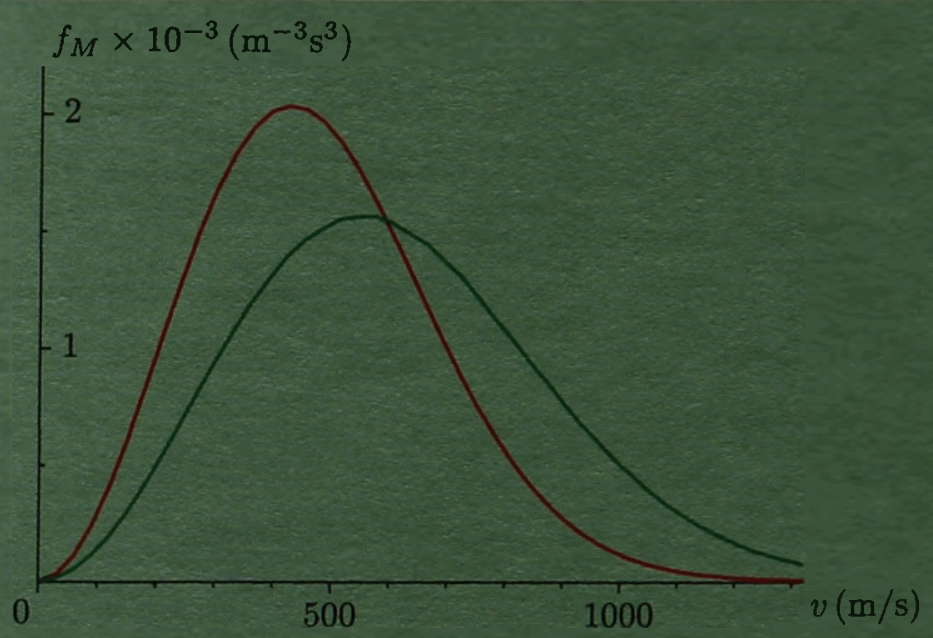
\includegraphics[width=0.4\linewidth]{mai_fig048.png}
   \captionof{figure}{Maxwellovo rozdělení rychlostí molekul dusíku pro teploty \(T_1 = 
                      \SI{300}{\kelvin}\) a \(T_2 = \SI{300}{\kelvin}\).
   \cite[s.~243]{Musilova2009MA1}
   \label{mai:fig048}}
  \par}
  
  Dokážete vyložit, proč jsme zvolili za \(\Delta\Omega\) celý objem slupky? Počítáme totiž 
  pravděpodobnost, že koncový bod vektoru rychlosti molekuly leží, zhruba řečeno, v kterémkoli 
  elementárním kvádříku \(\Delta v_x\Delta v_z\Delta v_z\) obsaženém ve slupce. A ta je součtem 
  pravděpodobností odpovídajících všem kvádříkům vytvářejícím slupku. Jedná se o pravděpodobnosti 
  navzájem neslučitelných jevů (pohybuje-li se molekula v jednom směru, nepohybuje se v jiném). 
  Hustota této pravděpodobnosti se nazývá \textbf{Maxwellovo rozdělení rychlostí}. Na rozdíl od 
  Gaussova rozdělení, popisujícího hustotu pravděpodobnosti pro jednotlivé složky rychlosti, je 
  nesymetrická vlivem faktoru \(v^2\). Obrázek \ref{mai:fig048} ukazuje funkci \(f_M(v)\) pro dvě 
  různé teploty \(T_2 > T_1\). Důležité hodnoty spjaté s tímto rozdělením jsou 
  \textbf{nejpravděpodobnější rychlost} \(v_p\), \textbf{střední rychlost} \(\langle v \rangle\) a 
  \textbf{střední kvadratická rychlost} \(\langle v^2 \rangle\). Platí
  \begin{align*}
    \der{f_M}{v}        &= 0\, \longrightarrow v_P = \sqrt{\dfrac{2kT}{m}},                      \\
    \langle v \rangle   &= \int_{-\infty}^{\infty}vf_M(v)\dd{v} = \sqrt{\dfrac{8kT}{\pi m}},     \\
    \langle v \rangle^2 &= \int_{-\infty}^{\infty}v^2f_M(v)\dd{v} = \dfrac{3kT}{m}
  \end{align*}
\normalsize
\end{example}